When the processing of the testing result is finished, the findings can be reported. This chapter is about the reporting of processed data. It will also touch on the visualization of the findings and using those visualisations to detect performance regressions.

As mentioned in Chapter 3, the choice of an appropriate performance metric is very important. When making a report, this is what it will be based around. A report based on CPU time will have a different structure than a report based on bandwidth. The performance metrics require additional data to be able to show regressions. This additional data can be the number of times the performance regression test has been executed or the number of times a particular function has been called. This kind of data can be useful in determining if a performance regression has occured. If a function is expected to be called twice as much since the last revision, an increase in performance can be expected.

\section{Visualisation}
When a report is created, a large amount of data can be useful. Only it is very hard and error prone to look over those numbers manually. Visualisation can be used to show the data in a way that might be easier to comprehend. This can be done by using visual representations, such as a graph, which can be used to spot a change in performance between revisions. There are different means of visualising the results of performance regression testing.

\subsection{Control Charts}
Control charts, which are explained in detail in Chapter 4, are a way to compare performance counters over two different revisions. It uses a prior revision as a baseline and sets a upper limit and lower limit. If the new data is within the limits, the performance of the revision is under control.
\begin{figure}[h]
\begin{center}
  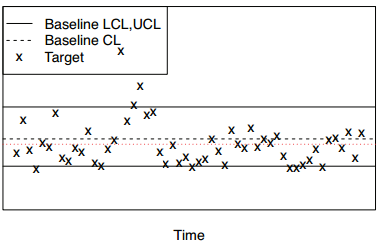
\includegraphics[scale=0.7]{Figures/controlchart.png}
\end{center}
  \caption{Example of a control chart\cite{nguyen2012using}.}
  \label{figure:control_chart}

\end{figure}

\subsection{Transaction Profile}
The transaction response time is the total time to process a request using the various system resources \cite{jain2008art}. The transaction profile represents the lower bound value of the transaction response time for a transaction. In other words, it is the transaction response time when the transaction is the only one in the system \cite{ghaith2015anomaly}. The transaction profile can be visualised using a bar graph. By comparing the bar graphs of two revisions of the software, it is possible to detect the regressions in performance.

\begin{figure}[h]
\begin{center}
  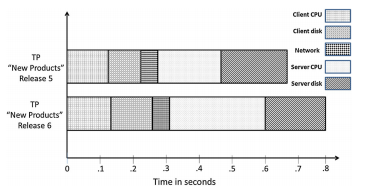
\includegraphics[width=0.5\textwidth]{Figures/TP.png}
\end{center}
  \caption{ Example of a transaction profile \cite{ghaith2015anomaly}.}

\end{figure}

The transaction profile consists of multiple components. It can be useful to compare each component seperately. Therefore, another way to visualise a transaction profile is to make separate bars for each component.

\begin{figure}[h]
\begin{center}
  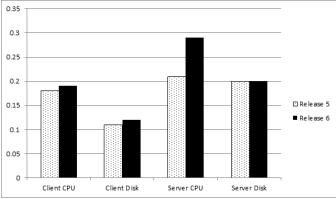
\includegraphics[width=0.5\textwidth]{Figures/TPbars.png}
\end{center}
  \caption{Example of a transaction profile divided into its components \cite{ghaith2015anomaly}.}

\end{figure}
\newpage
\subsection{Graphs}
The results of performance regression tests can also be represented in a normal graph. In this type of graph a lot of revisions can be visualised at once. Using this method gives a better overview of the performance of the system over entire project duration and not just over two particular revisions. This means you can look at 12 revisions, 50 revisions or even more. The following graph shows the number of written bytes for each revision of a software project.

\begin{figure}[h]
\begin{center}
  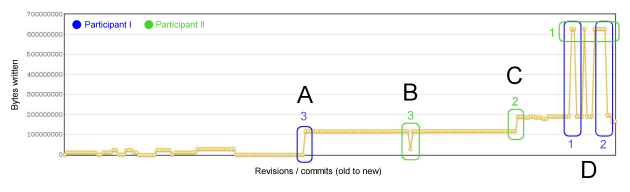
\includegraphics[width=0.5\textwidth]{Figures/bytegraph.png}
\end{center}
  \caption{The number of I/O write operations of a software system per revision \cite{bezemer2014detecting}.}

\end{figure}


\section{Reporting}
When not using visualisation, a report mostly consists of a table. This table contains information the developer has deemed most useful.
\begin{figure}[h]
\begin{center}
  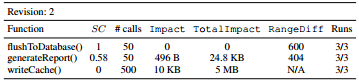
\includegraphics[width=0.5\textwidth]{Figures/table.png}
\end{center}
  \caption{A table with performance regression testing data \cite{bezemer2014detecting}.}

\end{figure}

 This can include the additional data, such as the number of test runs. Detecting regressions is done by analysing the report and finding a spike in performance. A spike in performance does not always mean there is a regression. It is possible that a new functionality is added, which can cause a spike in performance. Detecting regressions is not a discrete process. The measuring of performance is precarious. Because of the error-prone measurements, often a method that provides an accuracy along with each result. This shows how close to the previous revisions are to the new one.\\ \\


With the performance regressions visualised and reported, the developer can draw conclusions about the results. The visualisations give a quick overview of the performance of the program. Using this the developer can adjust their system quickly and more effectively than without this knowledge.


%\section{Detection of performance regressions}
%When a report and/or a visualization is created any regressions still have to be detected. Detecting regressions is done by analyzing the report and finding a spike in performance. A spike in performance does not always mean there is a regression. It is possible that new functionality is added, which can cause a spike in performance. Looking at the figure above a spike in performance can be seen indicated with an ``A''. ``Phenomenon A: The increase was caused by a bugfix. Before this bugfix, data was not committed to the database''\cite{bezemer2014detecting}.\newline
%Detecting regressions is not a discrete process. The measuring of performance is precarious. Because of the error-prone measurements, often a method that provides an accuracy measurement is used. This shows how close to the previous revisions are to the new one. To be more precise with this method it is best to run the tests a many times as possible. This is however impractical, because it could possibly take months or even longer. Because of this, in performace regression testing, the factor of time has to be weighed against the factor of accuracy.







%mogelijk report techniek: transaction profile
%http://onlinelibrary.wiley.com/doi/10.1002/stvr.1573/pdf
%average precision and recall
%http://sail.cs.queensu.ca/publications/pubs/qsic2010_foo.pdf
